\section{Introdução}

\subsection{Objeto de Estudo}
Esta apresentação irá tratar de um dispositivo de armazenamento de memória.

    \begin{figure}[H]
        \centering
        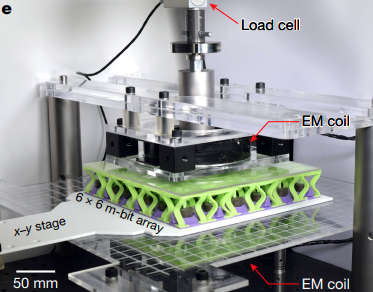
\includegraphics[scale = 0.5]{source/pictures/device.png}
        \caption{Imagem do dispositivo\cite{chen2021reprogrammable}.}
        \label{fig:device}
    \end{figure}

\subsubsection{O que é este dispositivo?}
    E um \textcolor{red}{dispositivo/sistema de memória} desenvolvido por Chen et al. capaz manipular informações de forma mecânica na estrutura do \textcolor{red}{material}\cite{coulais2021snappy}.\\ 

    Sendo capaz de:

    \begin{itemize}
        \item Codificar
        \item Armazenar
        \item Ler
        \item Alterar propriedades mecânicas do material
    \end{itemize}

    \textcolor{purple}{Para entendermos mais sobre este dispositivo, é necessário abordar os dois conceitos que envolvem este tema, que são: os metamateriais e os sistemas de armazenamento de dados. }

\subsection{Metamaterias}

\subsection{Sistemas de memória}
    \textcolor{purple}{Para melhor compreensão do funcionamento deste dispositivo, vamos construir uma analogia com outro dispositivo já conhecido que possui um funcionamento semelhante.}

\subsubsection{Discos Rigidos}

    \begin{figure}[H]
        \centering
        \includegraphics[scale = 0.5]}
        \caption{Imagem do dispositivo\cite{chen2021reprogrammable}.}
        \label{fig:device}
    \end{figure}